
\documentclass[letterpaper,11pt]{article}

\usepackage{style}
\usepackage{shortcuts}

\begin{document}
	
\begin{center}
	\begin{minipage}[H]{14.5cm} 
		
		\begin{center}
		{\huge \bf Near-Optimal Directed\\[.5ex]Low-Diameter Decompositions}
			\end{center}
		\vspace{1cm}
		
		{\large \textbf{Karl Bringmann}\footnote{This work is part of the project TIPEA that has received funding from the European Research Council (ERC) under the European Unions Horizon 2020 research and innovation programme (grant agreement No.~850979).} -- Saarland University and Max Planck Institute for Informatics, Saarland Informatics Campus, Germany} \vspace{1mm}\\
		{\large \textbf{Nick Fischer\footnote{Partially funded by the Ministry of Education and Science of Bulgaria's support for INSAIT as part of the Bulgarian National Roadmap for Research Infrastructure.}} -- INSAIT, Sofia University "St. Kliment Ohridski", Bulgaria} \vspace{1mm}\\
		{\large \textbf{Bernhard Haeupler\footnote{Partially funded by the Ministry of Education and Science of Bulgaria's support for INSAIT as part of the Bulgarian National Roadmap for Research Infrastructure and through the European Research Council (ERC) under the European Union's Horizon 2020 research and innovation program (ERC grant agreement 949272).}} -- INSAIT, Sofia University "St. Kliment Ohridski", Bulgaria \& ETH Zürich, Switzerland} \vspace{1mm}\\
		{\large \textbf{Rustam Latypov\footnote{Supported by the Research Council of Finland (grant 334238), The Finnish Foundation for Technology Promotion and The Nokia Foundation}} -- Aalto University, Finland} \vspace{1mm}\\


		\begin{abstract}
			\noindent
			Low Diameter Decompositions (LDDs) are invaluable tools in the design of combinatorial graph algorithms. While  historically they have been applied mainly to undirected graphs, in the recent breakthrough for the negative-length Single Source Shortest Path problem, Bernstein, Nanongkai, and Wulff-Nilsen [FOCS '22] extended the use of LDDs to directed graphs for the first time. Specifically, their LDD deletes each edge with probability at most \makebox{$O(\frac{1}{D} \cdot \log^2 n)$}, while ensuring that each strongly connected component in the remaining graph has a (weak) diameter of at most $D$.
			
			In this work, we make further advancements in the study of directed LDDs. We reveal a natural and intuitive (in hindsight) connection to Expander Decompositions, and leveraging this connection along with additional techniques, we establish the existence of an LDD with an edge-cutting probability of \makebox{$O(\frac{1}{D} \cdot \log n \log\log n)$}. This improves the previous bound by nearly a logarithmic factor and closely approaches the lower bound of \makebox{$\Omega(\frac{1}{D} \cdot \log n)$}. With significantly more technical effort, we also develop two efficient algorithms for computing our LDDs: a deterministic algorithm that runs in time~\smash{$\widetilde\Order(m \poly(D))$} and a randomized algorithm that runs in near-linear time~\smash{$\widetilde\Order(m)$}.

			We believe that our work provides a solid conceptual and technical foundation for future research relying on directed LDDs, which will undoubtedly follow soon.
		\end{abstract}
		
		\end{minipage}
	
\end{center}

\thispagestyle{empty}

%\newpage
%\thispagestyle{empty}
%\tableofcontents

\newpage
\pagenumbering{arabic}

% !TEX root = mfe.tex


\newcommand{\base}[1]{\ensuremath{\mathrm{#1}}\xspace}
\newcommand{\baseA}{\base{A}}
\newcommand{\baseT}{\base{T}}
\newcommand{\baseG}{\base{G}}
\newcommand{\baseC}{\base{C}}
\newcommand{\baseU}{\base{U}}

\section{Introduction}

The  {\em primary structure} of a DNA strand is simply a word   over the alphabet  $\{\baseA, \baseC, \baseG, \baseT\}$, or  $\{\baseA, \baseC, \baseG, \baseU\}$ for RNA.  
Bases may bond in pairs, \baseA binds to \baseT and \baseC binds to \baseG, and a set of such pairings for a strand is called a {\em secondary structure} as shown in {\cref{fig:sec struct}(a)}; typically each strand has exponentially many possible secondary structures.\footnote{A secondary structure, along with a set of experimental conditions,  induces one or more 3D structures called tertiary structures---a complication we will not be concerned with in this paper since, unlike proteins, it is fortunate that DNA/RNA interactions are sufficiently chemically simple that that somewhat elementary secondary structure model is sufficient for useful structural prediction.} 
Mainly, what practitioners care about are probabilities of a given secondary structure or class of secondary structures. 
For that, each secondary structure~$s$ has an associated, typically negative, real valued {\em free energy} $\Delta G(s)$, where more negative is deemed more favourable.  
Thus the most favourable is the secondary structure, or structures, with minimum free energy (MFE). 
More generally, the Boltzman distribution is  a probability distribution on secondary structures $s$ at chemical equilibrium:  
the probability of~$s$ is  $p(s) = \frac{1}{Z} \mathrm{e}^{- \Delta G(s)/k_\mathrm{B}T}  $ where $Z$ is a normalisation factor called the partition function: 
\begin{equation}\label{eq:pf}
	Z  = \sum_{s\in\Omega} \mathrm{e}^{- \Delta G(s)/k_\mathrm{B}T} 
\end{equation}
that is, an exponentially weighted sum of the free energies over the set~$\Omega$ of all secondary structures, 
where~$k_\mathrm{B}$ is Boltzmann's constant and $T$ is temperature in Kelvin. 

\begin{table}[t]
	\centering
	\begin{tabular}{ p{5cm}||p{5cm}|p{5cm}  }
		%\hline
		
		Input type& MFE & Partition function\\ 
		
		\hline\hline
		
		Single strand   &   $\mathcal{O}(N^4)$ \ \   \cite{zukeroptimal,zukerrna, nussinov1978algorithms, nussinov1980fast,waterman1986rapid}  &   $\mathcal{O}(N^4)$ \ \  \cite{mccaskill1990equilibrium}     \\  \hline
		Multiple strands, bounded,\newline i.e.~$c= \mathcal{O}(1)$ strands &  $\mathcal{O}(N^4 (c-1)!)$ \ \  {\bf [Theorem~\ref{thm:main}]}   &   $\mathcal{O}(N^4 (c-1)!)$  \ \ \  \cite{dirks2007thermodynamic}\footref{ft:N3}    \\ \hline
		Multiple strands, unbounded,\newline i.e.~$\mathcal{O}(N)$ strands &  APX-hard \ \   \cite{condon2021predicting}  &  Open problem   \\ \hline
	\end{tabular}\vspace{-1.5ex}
	\caption{\label{table}\small
		Some algorithmic results for MFE and partition function for unpseudoknoted\footref{ft:pseudoknot} nucleic acid systems.
		$N$ is the total number of bases of all strand(s) in the system (i.e.~sum of strand lengths).
		Results are shown for input being a single strand, 
		multiple strands bounded by a constant or unbounded/growing with~$N$. 
		Note that in the literature the polynomial is sometimes written to the power 3 (e.g.~$\mathcal{O}(N^3 ...)$), but this is for a restricted ``relaxation'' of the model.\footref{ft:N3}  
	}
\end{table}

Decades ago, the deep relationship between secondary structures and dynamic programming algorithms was established~\cite{zukeroptimal,zukerrna, nussinov1978algorithms, nussinov1980fast,waterman1986rapid, mccaskill1990equilibrium}.  
If a secondary structure can be drawn as a polymer graph  without edge crossings it is called unpseudoknotted  (\cref{fig:sec struct}(c)).
The earliest polynomial time algorithms were for single-stranded  unpseudoknotted secondary structures, with the absence of crossings allowing for planar decompositions of secondary structures that are suited  to dynamic programming techniques.\footnote{Exclusion of pseudoknots is usually founded on both modelling and algorithmic considerations. Energy models for pseudoknots are difficult to formulate due to the increased significance of geometric issues and tertiary interactions \cite{dirks2007thermodynamic}. If pseudoknots are permitted, it is known that the MFE prediction is NP-hard even for a single strand \cite{akutsu2000dynamic,lyngso2000pseudoknots,lyngso2000rna}.The first NP-hardness results \cite{akutsu2000dynamic,lyngso2000pseudoknots} used a simple energy model called the stacking model where only consecutive base pairs forming a stack contribute to the free energy of a secondary structure. These hardness results with relatively simple energy models, make it seems unlikely that the MFE prediction problem will be easier in the case of more complicated energy models~\cite{condon2021predicting}. But, dynamic programming algorithms are still possible for restricted classes of pseudoknots, for both MFE prediction \cite{rivas1999dynamic, uemura1999tree, chen2009n, jabbari2018knotty, reeder2004design} and partition function \cite{dirks2003partition, dirks2004algorithm}. \label{ft:pseudoknot}}  
For a single RNA/DNA strand, both MFE and partition function are computable in $\mathcal{O}(N^4)$ time (\cref{table}),  using the standard  energy model\footnote{This model is variably called the nearest neighbour model, the Turner model, and loop energy model. 
Versions of the model have been implemented in software suites such as NUPACK~\cite{dirks2007thermodynamic,dirks2004algorithm,fornace2020unified}, ViennaRNA~\cite{viennaRNA} and mfold~\cite{mfold}, for both RNA and DNA~\cite{santalucia1998unified,santa}.} that will be formally defined in \cref{sec:mfe}. 

Work in DNA computing~\cite{algoSST,squareRoot,cargoSorting,SIMDDNA,celltimer2017fernshulman,Chatterjee2017,seelig2006enzyme,zhang2011dynamic}, and nucleic acid nanotechnology more generally~\cite{geary2014single,woo2011programmable}, involves building molecular systems and structures with, to date, hundreds, and soon, thousands, of interacting strands, so there is a need for better algorithms for these multi-stranded `inverse design problems'~\cite{churkin2018design,nuad}.  
And, of course, biologists need to understand molecular structure in order to understand and predict molecular interactions. 
However, when there are multiple interacting strands, the situation becomes significantly more complicated than the single-stranded case for two reasons:  
First, for a secondary structure to be unpseudoknotted, it implies there should be {\em at least one} permutation of the strands without crossings on the polymer graph~\cite{dirks2007thermodynamic} (\cref{fig:sec struct}). 
Second, if strand types are repeated then 
so-called {\em rotational symmetries} (\cref{fig:sym}) arise that need to be accounted for in the model to match the underlying statistical mechanics\footnote{This fact from statistical mechanics is discussed in some papers~\cite{dirks2007thermodynamic,hofacker2012symmetric}, although we've not found its full derivation in the modern nucleic-acid algorithmic literature. We leave a first-principles derivation for future work.\label{ft:statmech}}, otherwise structures may be over- or undercounted, leading to incorrect probabilities in the Boltzmann distribution, in other words: incorrect predicted free energy of a secondary structure.

% A future version of this paper will include a

For multiple strands, albeit a constant number $c = \mathcal{O}(1)$, 
Dirks,  Bois, Schaeffer, Winfree and  
Pierce~\cite{dirks2007thermodynamic} gave a polynomial time partition function algorithm running in time $\mathcal{O}(N^4 (c-1)!)$.\footnote{We note that Dirks et al~\cite{dirks2007thermodynamic}, and others in field~\cite{zukeroptimal,zukerrna,condon2021predicting,waterman1986rapid,mccaskill1990equilibrium,boehmer2024rna}, often state the run time with 3  instead of 4 in the exponent (i.e. $\mathcal{O}(N^3)$ for single stranded and $\mathcal{O}(N^3 (c-1)!)$ for multistranded). This reduction comes from changing the standard energy model by putting some restrictions on the size of interior loops (\cref{fig:sec struct}), or by enforcing certain mild conditions on the energy parameters for the interior loops  \cite{lyngso1999fast,hofacker2012symmetric}, we do not assume these additional assumptions in this work.\label{ft:N3} Note that our time/space complexity could benefit from such model changes for example, via reduction of the upper bound in \cref{lem:polyub}}. 
The first problem goes away by simply assuming $c$ is a constant;
but if the number of strands is non-constant, in particular $c = \mathcal{O}(N)$, 
Codon, Hajiaghayi and Thachuk~\cite{condon2021predicting} showed MFE is NP-hard, and even APX-hard.\footnote{This hardness result holds whether or not rotational symmetries are accounted for in the energy model.} 
For the second, rotational symmetry, problem, in order to compute partition function, Dirks et al~\cite{dirks2007thermodynamic} found an algebraic link between the overcounting and the rotational symmetry correction problems, which allowed both to be solved simultaneously, aided by the exponential nature of the partition function.  
Surprisingly, that trick does not work for MFE:
Since MFE prediction is minimization-based, 
there is no secondary structure overcounting problem in MFE prediction---repeated secondary structures will not change the outcome of minimization, unlike the partition function which is summation-based.
Hence, the absence of the overcounting problem makes MFE prediction harder to solve, and was left open by Dirks et al~\cite{dirks2007thermodynamic}.
For the special case of two strands, Hofacker, Reidys, and Stadler~\cite{hofacker2012symmetric} gave an $\mathcal{O}(N^6)$  algorithm. In this paper, we propose an efficient solution to the $\mathcal{O}(1)$ strand MFE problem, the first that runs in polynomial time. 



\subsection{Statement of main result}
Our main result is the following theorem, whose proof is in \cref{sec:analysis}: 

\begin{restatable}{theorem}{main} 
	\label{thm:main}
	There is an $\mathcal{O}(N^4(c-1)!)$ time and $\mathcal{O}(N^4)$ space algorithm for the 
	Minimum Free Energy unpseudoknotted secondary structure prediction problem, including rotational symmetry, 
	for a set of $c = \mathcal{O}(1)$ DNA or RNA strands of  total length  $N$ bases. 
\end{restatable}

In \cref{sec:analysis} we give a time-space trade-off for our result, by showing a variation of the algorithm runs in $\mathcal{O}(N^4 \log N (c-1)!)$ time but $\mathcal{O}(N^3)$ space.  


We use the standard~\cite{dirks2007thermodynamic} definition of free energy (\cref{eq:DGss}) of multistranded unpseudoknotted secondary structures, which includes rotational symmetry, see \cref{sec:mfe} for formal definitions.  
We first give an extensive overview of the proof and paper structure, followed by future work. 


\begin{figure}[t]
	\centering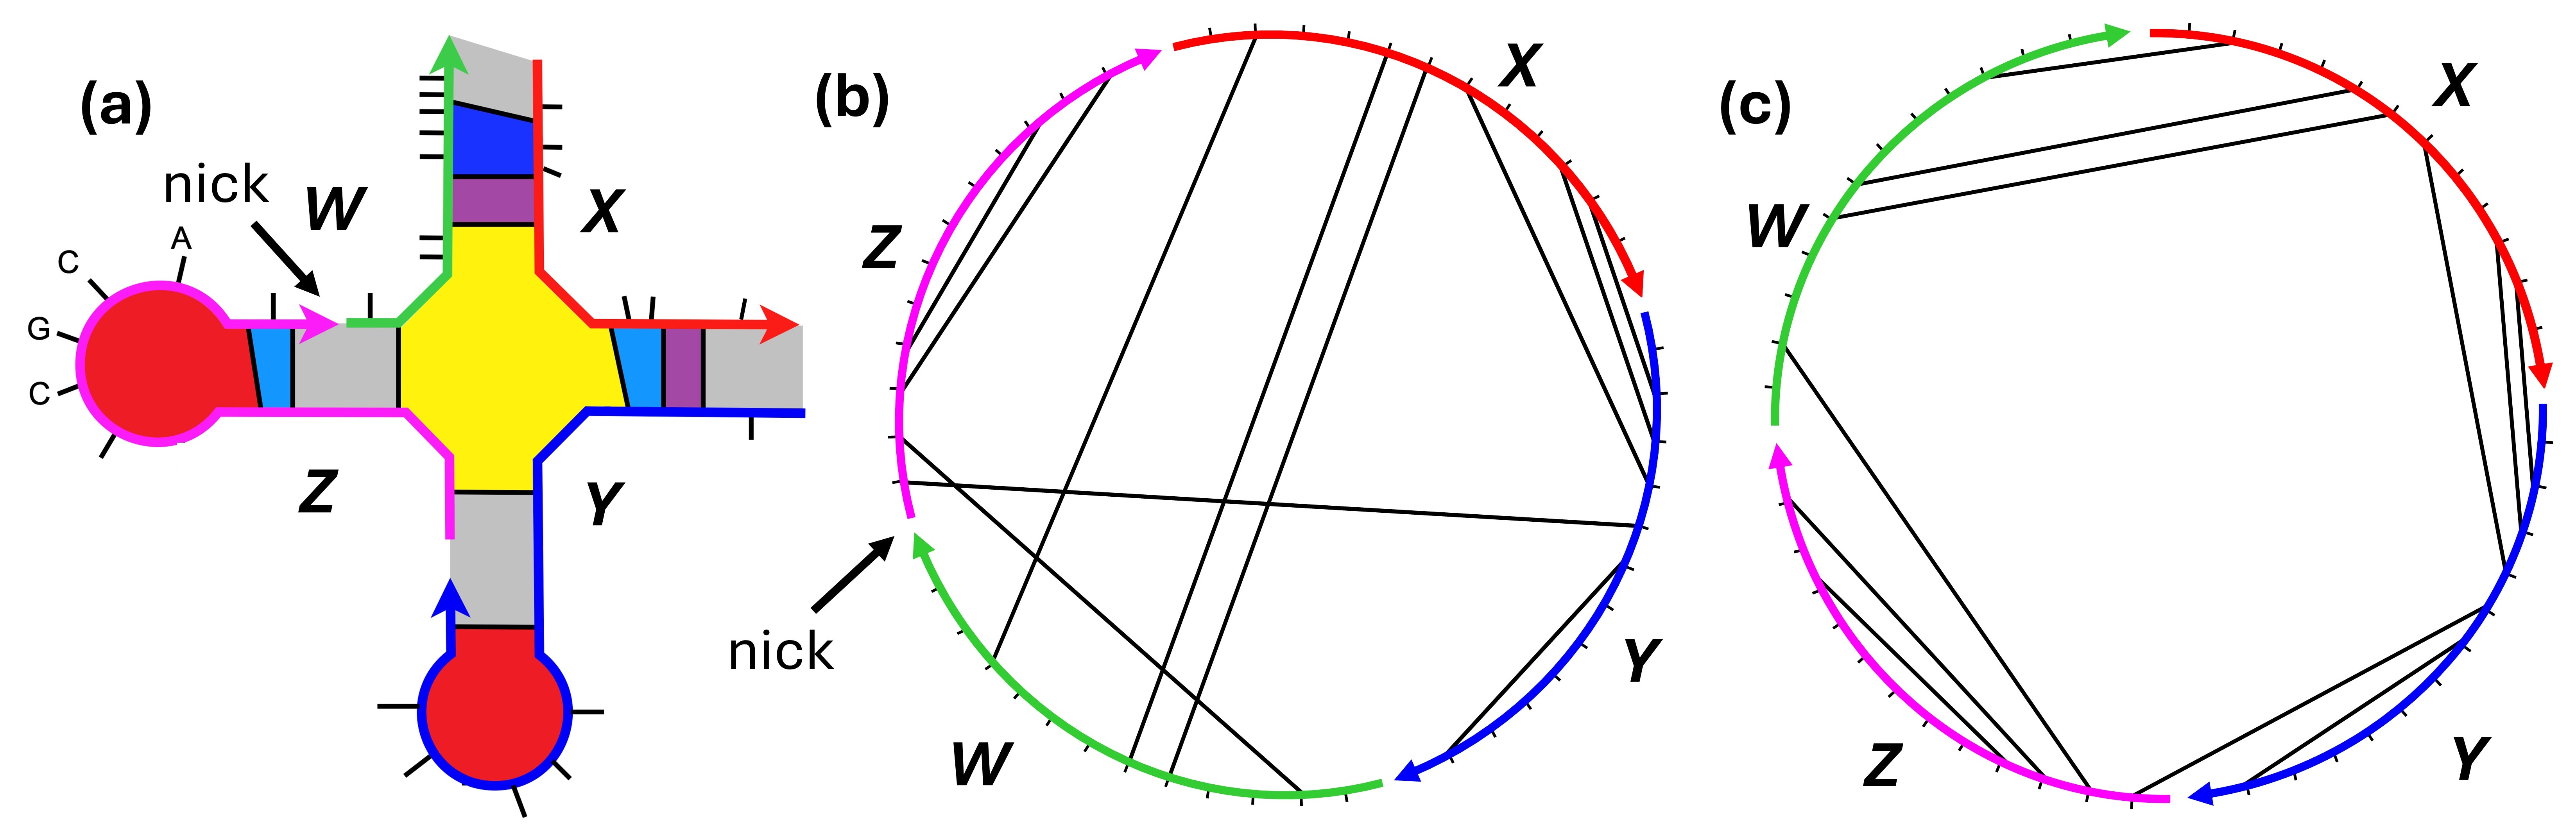
\includegraphics[width=0.9\textwidth]{figures/ss.jpg}
	\caption{
		A  DNA (or RNA) secondary structure $S$ with $c=4$ strands and two of its $(c-1)!=6$ polymer graphs. 
		(a) One of the many possible secondary structures for four DNA strands $W,X,Y,Z$. 
		Short black lines represent DNA bases (a few are shown $\ldots \baseC, \baseG, \baseC, \baseA \ldots$), and long lines represent base pairs (drawing not to scale). 
		Loops are colour-coded as follows:  stack=purple, multiloop=yellow, hairpin=red, bulge=light blue, internal=dark blue, external=grey.    
		Black arrow: the small gap between two strands is called a {\em nick}. 
		(b)~Polymer graph for the strand ordering $\pi' = WZXY$, denoted \PolySpiPrime, showing base-pair crossings.
		(c)~By  reordering to $\pi = WXYZ$ we get another polymer graph \PolySpi for $S$, without crossings, hence  $S$ is unpseudoknotted. 
	}
	\label{fig:sec struct}
	
\end{figure}

\subsection{Proof overview and paper structure}\label{sec:intuition}

\subsubsection{The main challenge: handling rotational symmetry}

Typically, each DNA base pair that forms represent a decrease (improvement in favourability) in free energy---although not always. 
In a multi-stranded system, when several strands bind together the entropy of the overall system is decreased since there are now less states due to their being less free molecules.  
Thus the energy model for multistranded systems includes an entropic {\em association penalty} (typically positive) for every extra strand, beyond the first, bound into a multistranded molecular  complex~\cite{dirks2007thermodynamic}. 
However, statistical mechanics tells us to be careful about symmetry: with multiple identical strands in a complex it is possible that the complex is rotationally symmetric, 
intuitively  there are several complexes, identical up to rotation of their polymer graphs (\cref{fig:sym}).\footnote{Formally, we mean the permutation representing the complex is rotationally symmetric.} 
These so-called indistinguishable complexes, in turn imply that a (positive) penalty should be applied to account for the difference in entropy between a similar, but distinguishable, complex without  rotational symmetry~\cite{bormashenko2019entropy,atkins2023atkins,silbey2022physical,fornace2020unified}.\footref{ft:statmech} 
\cref{sec:mfe} gives definitions needed  to formalise these concepts, including: DNA,  
unpseudoknotted secondary structure, polymer graph,  
free energy including rotational symmetry (\cref{eq:DGss}) and MFE (\cref{eq:MFE}). In particular, \cref{sec:sym} gives a  group-theoretic definition of rotational symmetry, to help formalise some of the prior work.

\subsubsection{General approach to find the true MFE}
One obvious idea might be to find a dynamic programming algorithm that directly handles rotational symmetry. 
However, this approache suffers from rotational symmetry being a {\em global property} of an entire system state (secondary structure), whereas dynamic programming relies on piecing together subproblems that are individually unaware of the global context---or more precisely, may be used in multiple global contexts whether symmetric or not.  

Instead, our strategy is to first compute what we call the {\em \symnMFE} (\snMFE) that (incorrectly) assumes all strands are distinct and thus does not compute correct free energies for rotational symmetries. 
We use  Dirks et al's \snMFE algorithm~\cite{dirks2007thermodynamic},  that assumes all strands are distinct, but  augmented to return extra dynamic programming matrices (\cref{algo:1} in \cref{sec:AlgoMFE}). 
We use these extra matrices to compute the required symmetry correction to that \snMFE value using a backtracking algorithm, as  follows.



\subsubsection{Polynomial upper bound: intuition for \cref{sec:ub}} 
Our goal is to show that, after running our augmentation of the known algorithm for \snMFE, we have implicit access to a collection of secondary structures that are `not too far' from the true MFE---where by `not too far' we mean we have a polynomial bound on the number of structures to be  considered by another fast (``backtracking'') algorithm that finds the true MFE structure.


First, 
to see how we find this polynomial bound,  imagine  the augmented
\snMFE algorithm finds that the secondary structure with \snMFE is  rotationally {\em  asymmetric}, hence we are done, we know that the \snMFE value is in fact the true MFE. 
Otherwise, we have a {\em rotationally symmetric} secondary structure: ideally we would like to compute it's rotational symmetry degree $R$ (takes linear time in the size of the secondary structure) and then return  $\mathrm{\snMFE} + k_\mathrm{B} T \log R$ as the true MFE, but this approach is doomed to fail since there could also be structures with lower true MFE, i.e.~in the real interval $[\mathrm{\snMFE}, \ \mathrm{\snMFE} + k_\mathrm{B} T \log R) \subset \mathbb{R}$. 



Leveraging the two properties of being (a) unpseudoknotted and (b) rotationally symmetric, in \cref{sec:ub} we define a class of cuts of a structure's polymer graph (\cref{fig:sec struct}) that we call {\em pizza cuts}, or, more formally, \emph{admissible symmetric backbone cuts} (\cref{def:admissible}). 
These cuts are radially symmetric, hence the name pizza cut---how one slices a pizza from disk-edge to centre.
In \cref{lem:ub,lem:ub2}, we show that there are at most a polynomial number of pizza cuts that symmetric structures may have. 



Then, when we do a backtracking-based search (below), 
through the dynamic programming matrices from the structure(s) with \snMFE, to larger free energies:  
if we find two different symmetric pizzas, but with the same pizza cuts,  we make a new pizza, by swapping a slice from one with a slice from the other.  
We prove that the new pizza is (a) guaranteed to be asymmetric and (b)~has free energy sandwiched between the {\snMFE} values of  two symmetric structures  (\cref{lem:sand,lem:ub2}). 
Moreover, this new structure's free energy is the true MFE. 
Otherwise we either find a symmetric structure (we output its naive free energy as the true MFE), or we reach a contradiction (i.e.~which can not happen) by reaching the polynomial bound having exhausted the set of all \emph{admissible symmetric backbone cuts}. In all cases the true MFE and its structure are output. 




\subsubsection{Backtracking to find the true MFE: intuition for \cref{sec:BT}} 

It remains to show how we will do the backtracking search mentioned above. 
In \cref{sec:BT} we analyse the  backtracking algorithm, which is given in \cref{algo:2} in \cref{app:backalgo}, and  
is a polynomial time  algorithm over the exponentially large set of structures `close' to the true MFE value. 
It scans all secondary structures within an energy level starting with the \symnMFE (\snMFE) energy level, it goes on to sequentially scan higher levels in low-to-high order. 
The scanning process at any energy level $\mathcal{E}$  guarantees that each secondary structure that belongs to $\mathcal{E}$ should be scanned exactly once. 

The backtracking algorithm will run until one of the following conditions occurs:
(1) It scans an asymmetric secondary structure $S$, or 
(2) it exceeds the polynomial upper bound $\mathcal{U}$ of the number of symmetric secondary structures (i.e. the number of distinct  pizza cuts) to be scanned, or 
(3) the backtracking will start scanning a new energy level $\mathcal{E}' > \mathcal{B}$, where $\mathcal{B}$ is the current best candidate for MFE (the starting value for $\mathcal{B}$ is  $\mathcal{B} = \mathrm{\snMFE} + k_\mathrm{B} \log v(\pi)$ where $v(\pi)$ is the highest degree of rotational symmetry, \cref{def:sym}). 
Then, based on the condition that will occur, the algorithm directly returns the true MFE, and a secondary structure which has the true MFE will also be constructed. 
The short proof of \cref{thm:main} in \cref{sec:analysis} ties these results together to give the final analysis of our main result.


\subsection{Future work}
Our algorithm runs in polynomial time $\mathcal{O}(N^4 (c-1)!)$ for the case of $c=\mathcal{O}(1)$ strands, the $(c-1)!$ term coming from the fact that our algorithm, as well as Dirks et al~\cite{dirks2007thermodynamic}, is assumed to be called from an outer  loop that explicitly tries all $(c-1)!$ cyclic strand permutations. 
Can we increase the number of strands and still have a polynomial time algorithm? We know ``not by much'', since the problem is NP-complete when $c=\mathcal{O}(N)$~\cite{condon2021predicting}. 
Interestingly, Boehmer, Berkemer, Will, and Ponty~\cite{boehmer2024rna} recently reduced the $c$-strand parameterized running time for computing \symnMFE (i.e.~ignoring rotational symmetry) and partition function from factorial, $\mathcal{O}(N^4 (c-1)!)$, to exponential, $\mathcal{O}(N^4  3^c)$.\footref{ft:N3}  
It is feasible that our MFE algorithm could be augmented via this result.

Our MFE algorithm exploits a polynomial upper bound, $\mathcal{U}$, on the number of so-called symmetric secondary structures, or distinct  pizza cuts.  That bound is linear in ``most'' cases (\cref{lem:even}), but quadratic in one special subcase (\cref{lem:ub2}) of 2-fold rotational symmetry with a central internal loop. Reducing  that special case to linear would subtract one from  our algorithm's running time exponent.

\cref{table} shows the open problem for partition function on multiple strands. Intuitively, it seems that  partition function should be at least as hard as MFE, however that intuition is tempered by the fact that Dirks et al's approach for partition function did not carry over to MFE, hence this is an open problem. Indeed, our paper brings extra techniques to handle multi-stranded MFE.   

More generally, the computational complexity of partition function for DNA/RNA strands is less well understood than MFE. 
For example, are there settings where partition function, or problems counting numbers of structures, are {\#}P-complete? 
\section{Results and Technical Overview} \label{sec:overview}
In a nutshell, our result is that we establish a directed LDD with \emph{near-optimal} loss $\Order(\log n \log\log n)$. This comes tantalizingly close to the unconditional lower bound of $\Omega(\log n)$. It resembles a similar milestone in the development of probabilistic tree embeddings~\cite{Bartal98}, and also the current state of the art for low-stretch spanning trees~\cite{AbrahamN19}. In fact, similar $\log\log n$ barriers show up also in different contexts for directed graphs~\cite{ChechikLRS20}. In a sense, all of these results with $\log\log n$ overhead (including ours) apply a careful recursive approach that can be traced back to work by Seymour~\cite{Seymour95} (though with strongly varying implementations depending on the setting). 

We state our result in three \cref{thm:main-existential,thm:main-det,thm:main-fast}, where the first theorem is purely existential, the latter two are algorithmic, and the last has \emph{near-linear} running time.

\subsection{Near-Optimal LDDs via Expander Decompositions} \label{sec:overview:sec:ldd-exp}
The main conceptual contribution of our paper is that Low-Diameter Decompositions are closely and in a very practical way related to Expander Decompositions. Based on this insight, we prove the following theorem.

\begin{restatable}{theorem}{thmMainExistential} \label{thm:main-existential}
	For every directed graph there exists a directed LDD with loss $O(\log n \log \log n)$.
\end{restatable}

For the remainder of \cref{sec:overview:sec:ldd-exp} we will elaborate on the proof of \cref{thm:main-existential}. It involves two separate steps: reducing the problem to \emph{cost-minimizing} using the \emph{Multiplicative Weight Update} method, and then showing that a so called \emph{lopsided} expander decomposition is the desired \emph{cost-minimizer}. We emphasize that in \cref{sec:overview:sec:ldd-exp} we only focus on Quest 1 from the introduction, which is minimizing the loss $L$ of an LDD.

\paragraph{Reduction to Unit Lengths.}
Let us assume throughout that we only deal with unit-length graphs (i.e., where $\ell(e) = 1$ for all edges). This assumption is in fact without loss of generality, as we can simply replace each edge $e$ of length $\ell(e)$ by a path of $\ell(e)$ unit-length edges. This transformation may blow up the graph, but as we focus on the existential result first this shall not concern us.\footnote{We are assuming throughout that all edge weights are bounded by $\poly(n)$, therefore this transformation leads to a graph on at most $n_0 \leq \poly(n)$ nodes. In particular, to achieve a loss of $L = \Order(\log n \log \log n)$ on the original graph it suffices to achieve a loss of $\Order(\log n_0 \log\log n_0)$ on the transformed graph.} Whenever the LDD cuts at least one of the path edges in the transformed graph, we imagine that the entire edge in the original graph is cut. This way, when we cut each edge with probability at most $\frac{L}{D}$, in the original graph we cut each edge with probability at most $\frac{\ell(e) \cdot L}{D}$ (by a union bound) as required.

\paragraph{Reduction to Cost-Minimization.}
Perhaps it appears surprising that we claim a connection between LDDs---which are inherently \emph{probabilistic} objects---and EDs---which rather have a \emph{deterministic} flavor. As a first step of bringing these notions together consider the following lemma based on the well-studied Multiplicative Weight Update \cite{AroraHazanKale12} method.
 

\begin{restatable}[Multiplicative Weight Update]{lemma}{mwu} \label{lem:mwu}
Let $G = (V, E)$ be a directed graph, and suppose that for all cost functions $c : E \to [|V|^{10}]$ there is a set of cut edges $S \subseteq E$ satisfying the following two properties:
\begin{itemize}
	\item For any two nodes $u, v \in V$ that are part of the same strongly connected component in $G \setminus S$, we have $d_G(u, v) \leq D$ and $d_G(v, u) \leq D$.
	\item $c(S) \leq c(E) \cdot \frac{L}{D}$.
\end{itemize}
Then there exists a directed LDD for $G$ with loss $\Order(L)$.
\end{restatable}

Intuitively, the lemma states that in order to construct an LDD that cuts each edge with small probability $L / D$, it suffices to instead find a cut which \emph{globally} minimizes the total cost of the cut edges while ensuring that every remaining strongly connected component has diameter at most~$D$. This however comes with the price of introducing a \emph{cost function $c$} to the graph, and the goal becomes to cut edges which collectively have at most an $L / D$ fraction of the total cost. For the reader's convenience, we include a quick proof sketch of \Cref{lem:mwu}.

\begin{proof}\textcolor{red}{TOPROVE 0}\end{proof}

Henceforth, we refer to the process of finding a cut with the properties stated in \Cref{lem:mwu} as a \emph{cost-minimizer}, which we aim to construct in the following paragraphs. That is, we now also consider a cost function $c$, and our goal is to cut edges $S$ of total cost~\smash{$c(S) \leq c(E) \cdot \frac{L}{D}$} (without worrying about a per-edge guarantee), while ensuring that the strongly connected components in~\makebox{$G \setminus S$} have diameter $\leq D$. We remark that this cost-minimization framework is quite standard.

\paragraph{Directed Expander Decomposition.}
In a leap forward, let us rename the \emph{costs $c$} to \emph{capacities~$c$}. Our idea is simple: We want to use an Expander Decomposition to remove edges of small total capacity so that all strongly connected components in the graph become expanders and thus, in particular, have small diameter.

To make this more precise, we first introduce some (standard) notation. A node set $U \subseteq V$ naturally induces a \emph{cut} (between $U$ and $\overline U = V \setminus U$). We write $c(U, \overline U)$ for the total capacity of edges crossing the cut from $U$ to $\overline U$, and define the \emph{volume} of $U$ as
\begin{equation*}
	\vol(U) = c(U, V) = \sum_{e \in E \cap (U \times V)} c(e),
\end{equation*}
and also write $\minvol(U) = \min\set{\vol(U), \vol(\overline U)}$. The \emph{sparsity} of the cut $U$ is defined by
\begin{equation*}
	\phi(U) = \frac{c(U, \overline U)}{\minvol(U)}.
\end{equation*}
We say that $U$ is \emph{$\phi$-sparse} if $\phi(U) \leq \phi$, and we call a graph without $\phi$-sparse cuts a \emph{$\phi$-expander.} The standard Expander Decomposition can be stated as follows.

\begin{lemma}[Directed Expander Decomposition] \label{lem:exp-decomp}
Let $\phi > 0$. For any directed graph $G = (V, E, c)$ there is an edge set $S \subseteq E$ of total capacity $c(S) \leq c(E) \cdot \phi \log c(E)$ such that every strongly connected component in the remaining graph $G \setminus S$ is a $\phi$-expander.
\end{lemma}

Moreover, an important property of a $\phi$-expander decomposition is that the diameter of its strongly connected components depends on $\phi$ in the following manner. 

\begin{lemma} \label{lem:exp-diam}
Any $\phi$-expander has diameter $\Order(\phi^{-1} \log \vol(V))$.
\end{lemma}

To understand the intuition behind \Cref{lem:exp-diam}, imagine that we grow a ball (i.e., a breadth-first search tree) around some node. With each step, the expansion property (related to the absence of $\phi$-sparse cuts) guarantees that we increase the explored capacity by a factor of $(1 + \phi)$; thus after $\Order(\phi \log \vol(V))$ steps we have explored essentially the entire graph.

Already at this point we have made significant progress and can recover the $\Order(\log^2 n)$-loss LDD: Apply the Expander Decomposition in \cref{lem:exp-decomp} with parameter $\phi = \log \vol(V) / D$. This removes edges with total capacity at most a $\Order(\log^2 \vol(V) / D)$-fraction of the total capacity. In the remaining graph each strongly connected component is a $\phi$-expander and thus, by \cref{lem:exp-diam}, has diameter at most $\Order(\phi^{-1} \log\vol(V)) = \Order(D)$ (by choosing the constants appropriately, this bound can be adjusted to~$\leq D$). Finally, \cref{lem:mwu} turns this into an LDD with loss $\Order(\log^2 \vol(V)) = \Order(\log^2 n)$.

Unfortunately, both log-factors in the Expander Decomposition (fraction of the cut capacity and diameter) are tight. Nevertheless, with some innovation we manage to bypass these bounds and improve the $\Order(\log^2 n)$ loss. To this end we propose a refined notion of expanders called \emph{lopsided expanders.}

\paragraph{Lopsided Expander Decomposition.}

The notion of $\phi$-sparsity defined above is oblivious to the ratio between $\vol(V)$ and $\minvol(U)$. For example, two cuts $U$ and $W$ can have the same sparsity, even though $\vol(U) \gg \vol(\overline U)$ while $\vol(W) \approx \vol(\overline W)$. It turns out that this leaves some unused potential, and that we should incentivize cutting cuts with large volume on both sides compared to more lopsided cuts with large volume only on one side.

Formally, we define \emph{$\psi$-lopsided sparsity} of a cut $U$ as 
\begin{align*}
	\psi(U) = \frac{c(U, \overline U)}{\minvol(U) \cdot \log \frac{\vol(V)}{\minvol(U)}},
\end{align*}
where we include the ratio~\smash{$\frac{\vol(V)}{\minvol(U)}$} in the denominator. Since $\vol(V)>\minvol(U)$, a cut can only have smaller lopsided sparsity than regular sparsity, so a graph with no sparse cuts may still have lopsided sparse cuts. A $\psi$-lopsided expander is defined as a graph with no $\psi$-lopsided sparse cuts, and can be thought of as a subclass of expanders which in addition to having no sparse cuts also has no cuts that are both sufficiently lopsided and sufficiently sparse.

The \emph{lopsided expander decomposition} is otherwise identical to the standard expander decomposition defined previously, except that every strongly connected component is required to be a \emph{$\psi$-lopsided} expander instead of a $\phi$-expander. Our Lopsided Expander Decomposition has the same global ``total capacity cut'' guarantee as the standard expander decomposition, as stated in the following lemma coupled with a proof sketch.

\begin{restatable}[Lopsided Expander Decomposition]{lemma}{lemLexpDecomp} \label{lem:lexp-decomp}
	Let $\psi > 0$. For any directed graph $G = (V, E, c)$ there is an edge set $S \subseteq E$ of total capacity $c(S) \leq c(E) \cdot \psi \log c(E)$ such that every strongly connected component in the remaining graph $G \setminus S$ is a $\psi$-lopsided expander.
\end{restatable}

\begin{proof}\textcolor{red}{TOPROVE 1}\end{proof}

The main motivation for defining $\psi$-lopsided sparsity and taking the ratio~\smash{$\frac{\vol(V)}{\minvol(U)}$} into account lies in the following lemma: Compared to standard expanders, lopsided expanders only suffer a loglog-factor in the diameter.

\begin{restatable}{lemma}{lemLexpDiam} \label{lem:lexp-diam}
	Any $\psi$-lopsided expander has diameter $\Order(\psi^{-1} \log \log \vol(V) + \log\vol(V))$.
\end{restatable}

\begin{proof}\textcolor{red}{TOPROVE 2}\end{proof}

Putting these two lemmas for lopsided expanders together, we indeed obtain the low-loss LDD in \Cref{thm:main-existential}. Specifically, we apply the Lopsided Expander Decomposition from \cref{lem:lexp-decomp} with parameter $\psi = \log\log \vol(V) / D$. We thereby cut only a $\Order(\log \vol(V) \log\log \vol(V) / D)$-fraction of the total capacity, and end up with a graph in which every strongly connected component is a $\psi$-lopsided expander. By \cref{lem:lexp-diam} said components have diameter $\Order(\psi^{-1} \log\log \vol(V)) = \Order(D)$ (which, again, can be made $\leq D$ by adjusting constants). Plugging this procedure into \cref{lem:mwu} we conclude that there is an LDD with loss $\Order(\log \vol(V) \log\log \vol(V)) = \Order(\log n \log\log n)$, completing the proof sketch of \cref{thm:main-existential}.

\subsection{A Deterministic Algorithm} \label{sec:overviewDet}
So far we have neglected Quest~2, i.e., the design of efficient algorithms. But how far from algorithmic is this approach of \Cref{sec:overview:sec:ldd-exp} really? It turns out that implementing this framework with some simple tricks leads to the following algorithmic result.

\begin{restatable}{theorem}{thmMainDet} \label{thm:main-det}
	For every directed graph there exists a directed LDD with loss $\Order(\log n \log\log n)$ and support size $\Order(D \log n)$ that can be computed in time $\widetilde\Order(m \poly(D))$ by a \emph{deterministic} algorithm.
\end{restatable}

This theorem comes with a strength and a weakness---the strength is that the theorem is deterministic. Note that the algorithm produces the \emph{explicit} support of an LDD; in fact, the probability distribution is simply a uniform distribution over a given list of cut sets $S$. For this reason, our algorithm might lead to some derandomized applications down the road by executing an LDD-based algorithm one-by-one for all $\Order(D \log n)$ cut sets. Derandomizations of this sort are common and sought after, especially in distributed and parallel domains. The weakness is that the running time has an overhead of $\poly(D)$. We remark that almost all algorithmic applications of LDDs (with the notable exception of~\cite{BernsteinNW22}) set $D = \polylog(n)$ or $D = n^{\order(1)}$, in which case the overhead is not dramatic, and the runtime is possibly near-linear.

\paragraph{Proof Idea.}
It can be quickly verified that implementing the Multiplicative Weights Update method from \Cref{lem:mwu} is not a problem algorithmically, and requires $O(R \cdot T)$ time, where $R=O(\log |E| \cdot D/L)$ and $T$ is the time required by the cost-minimizer. Hence, only computing the Lopsided Expander Decomposition could be costly. Since this is a strictly stronger definition that the standard Expander Decomposition, at first glance it appears hopeless that we could achieve a simple algorithm that avoids the cut-matching games machinery. Luckily, we find yet another simple insight that allows us to find a simple and intuitive algorithm after all: While it may generally be hard to find a sparse cut (even NP-hard!), in our case we only ever need to find a sparse cut \emph{in a graph with diameter more than $D$.} Indeed, if the graph has already diameter at most $D$, we can stop immediately (recall that we ultimately only care about the diameter and not the expander guarantee). One way to view the algorithm is that we construct a \emph{truncated} $\psi$-lopsided expander decomposition, where we terminate prematurely if the diameter is small.

Fueled by this insight, consider the following two-phase process for computing a (truncated) $\psi$-lopsided expander decomposition:
\begin{itemize}
    \setlength\parindent{1.6em}
    \setlength\parskip{0pt}
 	\item \emph{Phase (I):} We repeatedly take an arbitrary node $v$ and grow a ball around $v$ in the hope of finding a $\psi$-lopsided sparse cut. By choosing $\psi = \Theta(\log\log \vol(V) / D)$ we can guarantee two possible outcomes: 
 	\begin{enumerate}
 		\item[(a)] We find a sparse cut after, say, $\frac{D}{4}$ steps, in which case we cut the edges crossing the cut and recur on both sides (as in the Lopsided Expander Decomposition).
 		\item[(b)] The problematic case happens: the volume of the ball reaches $\frac{3}{4} \cdot \vol(V)$. In this case we have spent linear time but made no progress in splitting off the graph, so we remember $v$ and move to Phase (II).
 	\end{enumerate}
	
 	\item \emph{Phase (II):} We compute a \emph{buffer zone} around $v$, which consists of all nodes with distance $\frac{D}{2}$ to and from $v$. We repeatedly take an arbitrary node $u$ from outside this buffer zone and grow a ball around $u$ in the hope of finding a $\psi$-lopsided sparse cut. Because we know that the $\frac{D}{4}$-radius ball around $v$ contains most of the volume of the graph, and node $u$ is picked outside of the $\frac{D}{2}$-radius buffer zone, we can prove (using similar techniques to the proof sketch of \Cref{lem:lexp-diam}) that we will always find a $\psi$-lopsided sparse cut $U$ around $u$. Upon finding it, we cut the edges crossing the cut $(U, \overline U)$ and start Phase (I) for the graph induced by nodes in $U$, while continuing Phase (II) in graph $G \setminus U$.
 	
 	When eventually there are no nodes left outside the buffer zone, we stop, since the remaining graph has diameter $\leq D$.
\end{itemize}

The correctness of the procedure above is straightforward to show: we are essentially constructing a $\psi$-lopsided expander decomposition from \Cref{lem:lexp-decomp}, but terminating prematurely if the diameter is small. Hence, the total capacity of the cut edges is at most the total capacity of the cut edges in a ``complete'' $\psi$-lopsided expander, which is a $\Order(\log \vol(V) \log\log \vol(V) / D)$-fraction of the total capacity. The diameter guarantee follows directly from the stopping condition. By plugging this procedure into the algorithmic version of \cref{lem:mwu} we arrive at an LDD with loss $\Order(\log \vol(V) \log\log \vol(V)) = \Order(\log n \log\log n)$ in time $\widetilde\Order(m \poly(D))$, completing the proof sketch of \cref{thm:main-det}.


\subsection{A Near-Optimal Randomized Algorithm} \label{sec:overviewFast}

Our third and final contribution is achieving a near-linear running time, regardless of the magnitude of the diameter, by a randomized algorithm:

\begin{restatable}{theorem}{thmMainFast} \label{thm:main-fast}
	For every directed graph there exists a directed LDD with loss $\Order(\log n \log\log n)$ which can be computed (i.e., sampled from) in expected time $\widetilde\Order(m)$.
\end{restatable}

In contrast to \cref{thm:main-existential,thm:main-det}, our approach to \cref{thm:main-fast} is rather technical. We try more directly to extend the ideas of Bernstein, Nanongkai and Wulff-Nilsen~\cite{BernsteinNW22} (which in turn borrow ideas from~\cite{BernsteinGW20}). On a very high level, their algorithm classifies nodes $v$ \emph{heavy} if it reaches more than $\frac{n}{2}$ nodes within distance $\frac{D}{2}$, or \emph{light} otherwise. We can afford to cut around light nodes $v$ (with a specifically sampled radius $r \leq D$), and recur on both sides of the cut---since $v$ is light, the inside of the cut reduces by a constant fraction which is helpful in bounding the recursion depth. And if there are only heavy nodes in the graph then we can stop as the diameter is already at most $D$---indeed, the radius-$\frac{D}{2}$ balls around heavy nodes must necessarily intersect. The radius is sampled from a geometric distribution with rate $\Order(\log n / D)$ inspired by classical LDDs in undirected graphs~\cite{Bartal96}. The two logarithmic factors stem from (i) this $\log n$ overhead in the sampling rate, and (ii) the logarithmic recursion depth.

Our approach refines these ideas by classifying not into two classes---heavy or light---but into $\log\log n$ different levels. We essentially say that a node $v$ is at level $\ell$ if it reaches roughly $n / 2^{2^\ell}$ nodes within some distance roughly $D$. We can take advantage of this in two ways: At the one extreme, we can only cut around few nodes of small level $\ell$. Indeed, when we cut around a node at level $\ell$ we remove roughly $n / 2^{2^\ell}$ nodes from the graph, so this can be repeated at most $2^{2^{\ell}} \ll n$ times. For these levels we can afford to sample the radius in the geometric distribution with a significantly smaller rate, $\Order(2^i / D)$, thereby improving~(i). At the other extreme, whenever we cut around nodes with large level $\ell$ then in the recursive call of the inside of the cut there are only~$n / 2^{2^\ell} \ll n$ nodes. This effectively reduces the recursion depth of these levels to much less than $\log n$, improving (ii). In our algorithm, we find a balance between these two extreme cases. 

Unfortunately, while this idea works out existentially, there are several issues when attempting to implement this approach in near-linear time. The first issue---initially classifying which nodes are at what level in time $\widetilde\Order(m)$---can be solved by an algorithm due to Cohen~\cite{Cohen97}. However, over the course of the algorithm when we repeatedly remove nodes and edges from the graphs the level of a node might \emph{change}. Our solution involves a cute trick: First we prove that during the execution of our algorithm the level of a node can only \emph{increase} (and never decrease). Second, instead of cutting around an arbitrary node $v$, we always pick a \emph{random} node. The argument is as follows: If the classification is still correct for at least half of the nodes, then in each step we make progress with probability $\frac12$. And otherwise we can in fact afford to reclassify by Cohen's algorithm as the level of the nodes can only increase a small number of times, leading to only few repetitions of Cohen's algorithm in total.

We omit further details here and refer to the technical \cref{sec:ldd-fast}.
\section{Preliminaries} \label{sec:prelims}
Before diving into the technical results, we state the basic graph notations used throughout the paper and recap the new non-standard definitions we have introduced throughout \Cref{sec:overview}.

\paragraph{Graphs.}
Throughout we consider directed simple graphs $G = (V, E)$, where $E \subseteq V^2$, with $n = |V|$ nodes and $m = |E|$ edges. The edges of the graph can be associated with some value: a length $\ell(e)$ or a capacity/cost $c(e)$, all of which we require to be positive. For any $U \subseteq V$, we write $\overline U = V \setminus U$. Let $G[U]$ be the subgraph induced by $U$. We denote with $\delta^{+}(U)$ the set of edges that have their starting point in $U$ and endpoint in~$\overline U$. We define $\delta^{-}(U)$ symmetrically. We also sometimes write $c(S) = \sum_{e \in S} c(e)$ (for a set of edges $S$) or $c(U, W) = \sum_{e \in E \cap (U \times W)} c(e)$ and $c(U) = c(U, U)$ (for sets of nodes $U, W$).

The distance between two nodes $v$ and $u$ is written $d_G(v,u)$ (throughout we consider only the \emph{length} functions to be relevant for distances). We may omit the subscript if it is clear from the context. The diameter of the graph is the maximum distance between any pair of nodes. For a subgraph $G'$ of $G$ we occasionally say that~$G'$ has \emph{weak diameter} $D$ if for all pairs of nodes $u, v$ in~$G'$, we have $d_G(u, v), d_G(v, u) \leq D$. A strongly connected component in a directed graph $G$ is a subgraph where for every pair of nodes $v,u$ there is a path from $v$ to $u$ and vise versa. Finally, for a radius $r \geq 0$ we write $B^+(v, r) = \set{x \in V : d_G(v, x) \leq r}$ and $B^-(v, r) = \set{y \in V : d_G(y, v) \leq r}$.


\paragraph{Polynomial Bounds.}
For graphs with edge lengths (or capacities), we assume that they are positive and the maximum edge length is bounded by $\poly(n)$. This is only for the sake of simplicity in \cref{sec:ldd-expander,sec:ldd-deterministic} (where in the more general case that all edge lengths are bounded by some threshold $W$ some logarithmic factors in $n$ become $\log (nW)$ instead), and is not necessary for our strongest LDD developed in \cref{sec:ldd-fast}.

\paragraph{Expander Graphs.}
Let $G = (V, E, \ell, c)$ be a directed graph with positive edge capacities $c$ and positive unit edge lengths $\ell$. We define the \emph{volume $\vol(U)$} by
\begin{equation*}
	\vol(U) = c(U, V) = \sum_{e \in E \cap (U \times V)} c(e),
\end{equation*}
and set $\minvol(U) = \min\set{\vol(U), \vol(\overline U)}$ where $\overline U = V \setminus U$. A node set $U$ naturally corresponds to a cut $(U, \overline U)$. The \emph{sparsity} (or \emph{conductance}) of $U$ is defined by
\begin{equation*}
	\phi(U) = \frac{c(U, \overline U)}{\minvol(U)}.
\end{equation*}
In the special cases that $U = \emptyset$ we set $\phi(U) = 1$ and in the special case that $U \neq \emptyset$ but $\vol(U) = 0$, we set $\phi(U) = 0$.
We say that $U$ is \emph{$\phi$-sparse} if $\phi(U) \leq \phi$. We say that a directed graph is a $\phi$-expander if it does not contain a $\phi$-sparse cut $U \subseteq V$. 
We define the \emph{lopsided sparsity} of $U$ as
\begin{equation*}
	\psi(U) = \frac{c(U, \overline U)}{\minvol(U) \cdot \log \frac{\vol(V)}{\minvol(U)}},
\end{equation*}
(with similar special cases), and we similarly say that $U$ is \emph{$\psi$-lopsided sparse} if $\psi(U) \leq \psi$. Finally, we call a graph a \emph{$\psi$-lopsided expander} if it does not contain a $\psi$-lopsided sparse cut $U \subseteq V$.

\section{Near-Optimal LDDs via Expander Decompositions} \label{sec:ldd-expander}

In this section, we show the existence of a near-optimal LDD, thereby proving our first main theorem: 

\thmMainExistential*

We introduce some technical lemmas in order to build up the framework for the proof of \Cref{thm:main-existential}, which can be found in the end of the section.


\subsection{Reduction to Cost-Minimizers}

\mwu*

\begin{proof}\textcolor{red}{TOPROVE 0}\end{proof}

\lemLexpDecomp*

\begin{proof}\textcolor{red}{TOPROVE 1}\end{proof}

To prove that lopsided expanders have small diameter, we first establish the following technical lemma. 

\begin{lemma} \label{lem:lopsided-expansion}
Let $G = (V, E, c)$ be a directed graph and let $\psi > 0$. For any node $v \in V$ there is some radius $R = \Order(\psi^{-1} \log\log \vol(V) + \log \vol(V))$ such that one of the following two properties holds:
\begin{itemize}
	\item $\vol(B^+(v, R)) \geq \frac{1}{2} \cdot \vol(V)$, or
	\item $\psi(B^+(v, r)) \leq \psi$ for some $0 \leq r \leq R$.
\end{itemize}
\end{lemma}
\begin{proof}\textcolor{red}{TOPROVE 2}\end{proof}

One can easily strengthen the lemma as follows. This insight will play a role in the next \cref{sec:ldd-deterministic} in the construction of the deterministic algorithm.

\begin{lemma} \label{lem:lopsided-expansion-boosted}
Let $G = (V, E, c)$ be a directed graph and let $\psi > 0$ and $0 < \alpha < 1$. For any node $v \in V$ there is some radius $R = \Order(\psi^{-1} \log\log \vol(V) + \psi^{-1} \alpha^{-1} + \log \vol(V))$ such that one of the following two properties holds:
\begin{itemize}
	\item $\vol(B^+(v, R)) \geq (1 - \alpha) \cdot \vol(V)$, or
	\item $\psi(B^+(v, r)) \leq \psi$ for some $0 \leq r \leq R$.
\end{itemize}
\end{lemma}
\begin{proof}\textcolor{red}{TOPROVE 3}\end{proof}

\lemLexpDiam*

\begin{proof}\textcolor{red}{TOPROVE 4}\end{proof}

\begin{proof}\textcolor{red}{TOPROVE 5}\end{proof}
\section{Near-Optimal LDDs Deterministically} \label{sec:ldd-deterministic}
In this section, we present the deterministic algorithm for computing a near-optimal LDD, thereby proving our second main theorem:

\thmMainDet*

To this end, we utilize many of the same building blocks we have already introduced in \Cref{sec:ldd-expander}. In particular, we follow the general framework of Multiplicative Weights Update to reduce the computation of an LDD to solving the cost-minimizing task. The full proof of \Cref{thm:main-det} can be found in the end of the section. The following lemma restates the MWU method algorithmically; we omit a proof as it follows exactly the proof of \cref{lem:mwu} in \Cref{sec:ldd-expander}. 

\begin{lemma}[Algorithmic Multiplicative Weight Update]
Let $G = (V, E)$ be a directed graph and let $D \geq 1$. Suppose that there is an algorithm $\mathcal A$ that, given $G$, $D$ and a cost function $c : E \to [|V|^{10}]$, computes a set of edges $S \subseteq E$ satisfying the following properties:
\begin{itemize}
	\item For any two nodes $u, v \in V$ that are part of the same strongly connected component in $G \setminus S$, we have $d_G(u, v) \leq D$ and $d_G(v, u) \leq D$.
	\item $c(S) \leq c(E) \cdot \frac{L}{D}$.
\end{itemize}
Then there is a deterministic algorithm to compute an LDD with loss $\Order(L)$ for $G$ (i.e., we compute the full support of a uniform distribution over $\Order(D \log n)$ cut sets). It runs in time~\smash{$\widetilde\Order(m D)$} and issues $\Order(D \log n)$ oracle calls to $\mathcal A$.
\end{lemma}

For the remainder of this section we will therefore focus on the same cost minimizer setting: Given a directed graph $G = (V, E, c)$ with edge capacities (and unit lengths), the goal is select a set of cut edges $S \subseteq E$ such that $c(S) \leq c(E) \cdot \Order(\frac{1}{D} \cdot \log n \log\log n)$ and such that all strongly connected components in the remaining graph $G \setminus S$ have (weak) diameter at most $D$.

The following lemma is a consequence of the lopsided expander machinery set up before:

\begin{lemma}[Finding Sparse Cuts] \label{lem:sparse-cut-det}
Let $G = (V, E, c)$ be a directed graph, let $D \geq \log \vol(V)$ and let $v \in V$. Then there is some $\psi = \Order(\frac{1}{D} \cdot \log\log \vol(V))$ and an algorithm to determine which of the following cases applies:
\begin{enumerate}[label=(\roman*)]
	\item There is a radius $0 \leq r \leq D$ with $\psi(B^+(v, r)) \leq \psi$ and $c(B^+(v, r)) \leq 0.95 \cdot \vol(V)$.\\(In this case the algorithm runs in linear time in the number of edges incident to $B^+(v, r)$.)
	\item Or, there is a radius $0 \leq r \leq D$ such that $\psi(\overline{B^-(v, r)}) \leq \psi$ and $c(B^-(v, r)) \leq 0.95 \cdot \vol(V)$.\\(In this case the algorithm runs in linear time in the number of edges incident to $B^-(v, r)$.)
	\item Or, $c(B^+(v, D) \cap B^-(v, D)) \geq 0.9 \cdot \vol(V)$.\\(In this case the algorithm runs in time~\smash{$\Order(m)$}.)
\end{enumerate}
\end{lemma}
\begin{proof}\textcolor{red}{TOPROVE 0}\end{proof}

Having established \cref{lem:sparse-cut-det}, now consider the algorithm in \cref{alg:det}. In summary, it runs in two phases. In Phase (I) we first repeatedly select a node $v$ and attempt to cut a lopsided sparse cut around $v$ (i.e., we cut the edges in $\delta^+(B^+(v, r))$ for some radius $r$). We only execute these cuts, however, until we find a node $z$ for which $c(B^+(z, D') \cap B^-(z, D')) \geq 0.9 \cdot \vol(V)$---that is, both the radius-$D'$ out- and in-balls of $z$ make up for a big constant fraction of the entire graph. We call $z$ a \emph{center} node and move on to phase (II). In this phase we repeat the same steps as in Phase (I), but we only choose nodes $v$ that have distance at least $2D'$ (in one direction or the other) to the center $z$. The intuition is that we can never find a second node $z'$ which equally makes up for the entire graph, as then $z$ and $z'$ would have to be connected by a short path. In the remainder of this section we formally analyze \cref{alg:det}.

\begin{algorithm}[t]
	\caption{The deterministic near-optimal LDD, see \Cref{thm:main-det}.} \label{alg:det}
	\begin{enumerate}[label=\arabic*.]
		\item[(I)] Repeat the following steps: Take an arbitrary node $v \in V$ and apply \cref{lem:sparse-cut-det} with parameter \smash{$D' = \floor{\frac{D}{4}}$}. Depending on the output execute the following steps:
		\begin{enumerate}[label=(\roman*)]
			\item Cut all edges in $\delta^+(B^+(v, r))$, recurse on the induced graph $G[B^+(v, r)]$, then remove all nodes in $B^+(v, r)$ from the graph.
			\item Cut all edges $\delta^-(B^-(v, r))$, recurse on the induced graph $G[B^-(v, r)]$, then remove all nodes in $B^-(v, r)$ from the graph.
			\item Remember $z \gets v$ (called the \emph{center} node) and continue with Phase (II).
		\end{enumerate}
		\item[(II)] Compute the sets
		\begin{align*}
			X &= B^+(z, D') \cap B^-(z, D'), \\
			Y &= B^+(z, 2D') \cap B^-(z, 2D').
		\end{align*}
		Then repeat the following steps while there still exists nodes in $V \setminus Y$: Take an arbitrary node~\makebox{$u \in V \setminus Y$} and apply \cref{lem:sparse-cut-det} with parameter~$D'$. Depending on the output execute the following steps:
		\begin{enumerate}[label=(\roman*)]
			\item Cut all edges in $\delta^+(B^+(v, r))$, recurse on the induced graph $G[B^+(v, r)]$, then remove all nodes in $B^+(v, r)$ from the graph.
			\item Cut all edges $\delta^-(B^-(v, r))$, recurse on the induced graph $G[B^-(v, r)]$, then remove all nodes in $B^-(v, r)$ from the graph.
		\end{enumerate}
	\end{enumerate}
\end{algorithm}

\begin{lemma}[Total Cost of \cref{alg:det}] \label{lem:ldd-det-cost}
Let $S \subseteq E$ denote the set of edges cut by \cref{alg:det}. Then $c(S) \leq c(E) \cdot \Order(\frac{1}{D} \cdot \log \vol(V) \log\log \vol(V))$.
\end{lemma}
\begin{proof}\textcolor{red}{TOPROVE 1}\end{proof}

\begin{lemma}[Well-Definedness of \cref{alg:det}] \label{lem:ldd-det-well-defined}
While executing Phase~(II) of \cref{alg:det}, the subcase~(iii) never happens.
\end{lemma}
\begin{proof}\textcolor{red}{TOPROVE 2}\end{proof}

\begin{lemma}[Correctness of \cref{alg:det}] \label{lem:ldd-det-correctness}
Let $S \subseteq E$ denote the set of edges cut by \cref{alg:det}. Then for any two nodes $u, w$ in the same strongly connected component in $G \setminus S$, it holds that $d_G(u, w) \leq D$ and $d_G(w, u) \leq D$.
\end{lemma}
\begin{proof}\textcolor{red}{TOPROVE 3}\end{proof}

\begin{lemma}[Running Time of \cref{alg:det}] \label{lem:ldd-det-time}
\cref{alg:det} runs in time $\Order(m \log \vol(V))$.
\end{lemma}
\begin{proof}\textcolor{red}{TOPROVE 4}\end{proof}

This completes the analysis of \cref{alg:det} and puts us in the position of completing the proof of \cref{thm:main-det}.

\begin{proof}\textcolor{red}{TOPROVE 5}\end{proof}
\section{Near-Optimal LDDs in Near-Linear Time} \label{sec:ldd-fast}
In this section we show that near-optimal LDDs can even be computed in near-linear (i.e., near-optimal) running time. Formally, the goal of this section is to prove the last of our main theorems:

\thmMainFast*

We structure this section as follows: In \cref{sec:ldd-fast:sec:cutting} we first prove an important cutting lemma (\cref{lem:cut-light}), which we then apply in \cref{sec:ldd-fast:sec:algo} to prove \cref{thm:main-fast}.

\subsection{Cutting Lemma} \label{sec:ldd-fast:sec:cutting}
We rely on the following result due to Cohen that we can approximate efficiently the sizes of out-balls $\Bout(v, r)$ simultaneously for all nodes $v$. Note that we can equally approximate the size of the in-balls $\Bin(v, r)$ by applying \cref{lem:cohen} on the reverse graph.

\begin{lemma}[Cohen's Algorithm~{{\cite[Theorem~5.1]{Cohen97}}}] \label{lem:cohen}
Let $G$ be a directed weighted graph, let $r \geq 0$ and~\makebox{$\epsilon > 0$}. There is an algorithm that runs in time $\Order(m \epsilon^{-2} \log^3 n)$ and computes approximations~$b(v)$ satisfying with high probability that
\begin{equation*}
    (1 - \epsilon) |\Bout(v, r)| \leq b(v) \leq (1 + \epsilon) |\Bout(v, r)|.
\end{equation*}
\end{lemma}

The goal of this subsection is to establish the following lemma:

\begin{lemma}[Cutting Light Nodes] \label{lem:cut-light}
Let $G = (V, E)$ be a directed weighted graph, and consider the parameters $\delta > 0$, $0 \leq r_0 < r_1$, $1 \leq s_1 < s_0 \leq m$. There is an algorithm that computes a set of cut edges $S \subseteq E$ and sets of remaining vertices $R \subseteq V$ such that:
\begin{enumerate}[label=(\roman*)]
    \item Each strongly connected component in $G \setminus S$ either only contains nodes from $R$ or only nodes from $V \setminus R$. In the latter case it contains at most $\frac32 \cdot \frac{m}{s_1}$ edges.
    \item For every node $v \in R$ with $|\Bout_G(v, r_1)| \leq \frac{m}{s_1}$, it holds that $|\Bout_{G[R]}(v, r_0)| \leq \frac{m}{s_0}$.
    \item None of the edges in $S$ has its source in $R$ (i.e., $S \subseteq (V \setminus R) \times V$). Moreover, for each edge $e = (x, y) \in E$ it holds that:
    \begin{equation*}
        \Pr(e \in S \mid x \not\in R) \leq \frac{w_e \ln(2s_0 / \delta)}{r_1 - r_0}.
    \end{equation*}
\end{enumerate}
With probability at most $\delta$ the algorithm instead returns ``fail'', and with probability at most~$\frac{1}{\poly(n)}$ the algorithm returns an arbitrary answer. The running time is~\smash{$\Order(m \log^4 n)$}.
\end{lemma}

\begin{proof}\textcolor{red}{TOPROVE 0}\end{proof}

\subsection{Near-Linear-Time LDD} \label{sec:ldd-fast:sec:algo}
We are ready to state the LDD algorithm. Throughout this section, we fix the following parameters:
\begin{itemize}
    \item $L = \ceil{\log\log m} + 1$,
    \item \smash{$\delta = \frac{1}{\log^{10} m}$},
    \item $r_0 := 0$ and \smash{$r_\ell := r_{\ell-1} + \frac{D}{2^{L-\ell+3}} + \frac{D}{4 L}$} (for $1 \leq \ell \leq L$),
    \item \smash{$s_\ell := \min(2^{2^{L-\ell}}, m+1)$} (for $0 \leq \ell \leq L$).
\end{itemize}
With these parameters in mind, consider \cref{alg:ldd-fast}. The algorithm first deletes all edges with sufficiently large weight. Then it proceeds in $L$ iterations where in each iteration we apply \cref{lem:cut-light} to cut some edges in the graph (or reverse graph). If any of these calls returns ``fail'', then the entire algorithm restarts. In the following \cref{lem:ldd-fast-correctness,lem:ldd-fast-prob,lem:ldd-fast-time} we will show that this procedure correctly implements the algorithm claimed in \cref{thm:main-fast}.

\begin{algorithm}[t]
\caption{The near-linear-time near-optimal LDD, see \cref{thm:main-fast}.} \label{alg:ldd-fast}
\begin{enumerate}
    \item Initially let $S \subseteq E$ be the set of edges of weight at least $\frac{D}{4L}$, and remove these edges from $G$
    \item For $\ell \gets L, \dots, 1$:
    \begin{enumerate}
        \item[2.1.] Run \cref{lem:cut-light} on $G$ with parameters $\delta, r_{\ell-1}, r_\ell, s_{\ell-1}, s_{\ell}$, and let $S^+_\ell, R^+_\ell$ denote the resulting sets.
        \item[2.2.] Compute the strongly connected components in $(G \setminus S^+_\ell)[V \setminus R^+_\ell]$. Recur on each such component and add the recursively computed cut edges to $S$.
        \item[2.3.] Update $G \gets G[R^+_\ell]$ and $S \gets S \cup S^+_\ell$.
        \item[2.4.] Run \cref{lem:cut-light} on $\rev(G)$ with parameters $\delta, r_{\ell-1}, r_\ell, s_{\ell-1}, s_{\ell}$, and let $S^-_\ell, R^-_\ell$ denote the resulting sets.
        \item[2.5.] Compute the strongly connected components in $(G \setminus S^-_\ell)[V \setminus R^-_\ell]$. Recur on each such component and add the recursively computed cut edges to $S$.
        \item[2.6.] Update $G \gets G[R^-_\ell]$ and $S \gets S \cup S^-_\ell$.
    \end{enumerate}
    \item If any of the $2L$ previous calls to \cref{lem:cut-light} returns ``fail'', then we restart the entire algorithm (i.e., we reset $G$ to be the given graph, we reset $S \gets \emptyset$, and we start the execution from step~1).
\end{enumerate}
\end{algorithm}

\begin{lemma}[Correctness of \cref{alg:ldd-fast}] \label{lem:ldd-fast-correctness}
Let $u, v$ be two nodes lying in the same strongly connected component in $G \setminus S$. Then $d_G(u, v) \leq D$.
\end{lemma}
\begin{proof}\textcolor{red}{TOPROVE 1}\end{proof}

\begin{lemma}[Edge Cutting Probability of \cref{alg:ldd-fast}] \label{lem:ldd-fast-prob}
For any edge $e \in E$, we have
\begin{equation*}
    \Pr(e \in S) \leq \Order\parens*{\frac{w_e}{D} \cdot \log n \log\log n + \frac{1}{\poly(n)}}.
\end{equation*}
\end{lemma}
\begin{proof}\textcolor{red}{TOPROVE 2}\end{proof}

\begin{lemma}[Running Time of \cref{alg:ldd-fast}] \label{lem:ldd-fast-time}
The expected running time is $\Order(m \log^5 n \log\log n)$.
\end{lemma}
\begin{proof}\textcolor{red}{TOPROVE 3}\end{proof}

We remark that we have not attempted to optimize the log-factors in the running time here and it is likely that the overhead can be reduced. An obvious improvement to shave one log-factor from the running time is to employ a faster priority queue in Dijkstra's algorithm, e.g.\ as developed by Thorup~\cite{Thorup03}.
\bibliographystyle{plainurl}
\bibliography{ref}

\end{document}
